\documentclass[10 pt,usenames,dvipsnames, oneside]{article}
\usepackage{../../modelo-fracoes}
\graphicspath{{../../../Figuras/licao05/}}


\begin{document}

\begin{center}
  \begin{minipage}[l]{3cm}

\includegraphics[width=2cm]{../../../Figuras/logo}       
\end{minipage}\hfill
\begin{minipage}[r]{.8\textwidth}
 {\Large \scshape Atividade: }  
\end{minipage}
\end{center}
\vspace{.2cm}

\ifdefined\prof
%Caixa do Para o Professor
\begin{goals}
%Objetivos específicos
\begin{enumerate}
    \item       Comparar, somar e subtrair frações a partir da determinação de um denominador comum com base no processo geométrica de subdivisão da unidade;
    \item       Explorar as interpretações de juntar para a adição e de comparar para a subtração.

\end{enumerate}

\tcblower

%Orientações e sugestões
\begin{itemize}
    \item       Considere que, como na \hyperref[chap5-ativ13]{atividade 13}, é explorada aqui a noção de fração como parte de uma unidade em uma situação contextualizada, com as interpretações de juntar para a adição e de comparar para a subtração, agora com três parcelas e com uma situação envolvendo volume.
\end{itemize}
\end{goals}

\bigskip
\begin{center}
{\large \scshape Atividade}
\end{center}
\fi

Há três recipientes cilíndricos, de mesmo tamanho, contendo água. No primeiro recipiente, a água ocupa dois terços de sua capacidade. No segundo, a água ocupa metade de sua capacidade. No terceiro, a água ocupa cinco oitavos de sua capacidade.

\begin{center}
  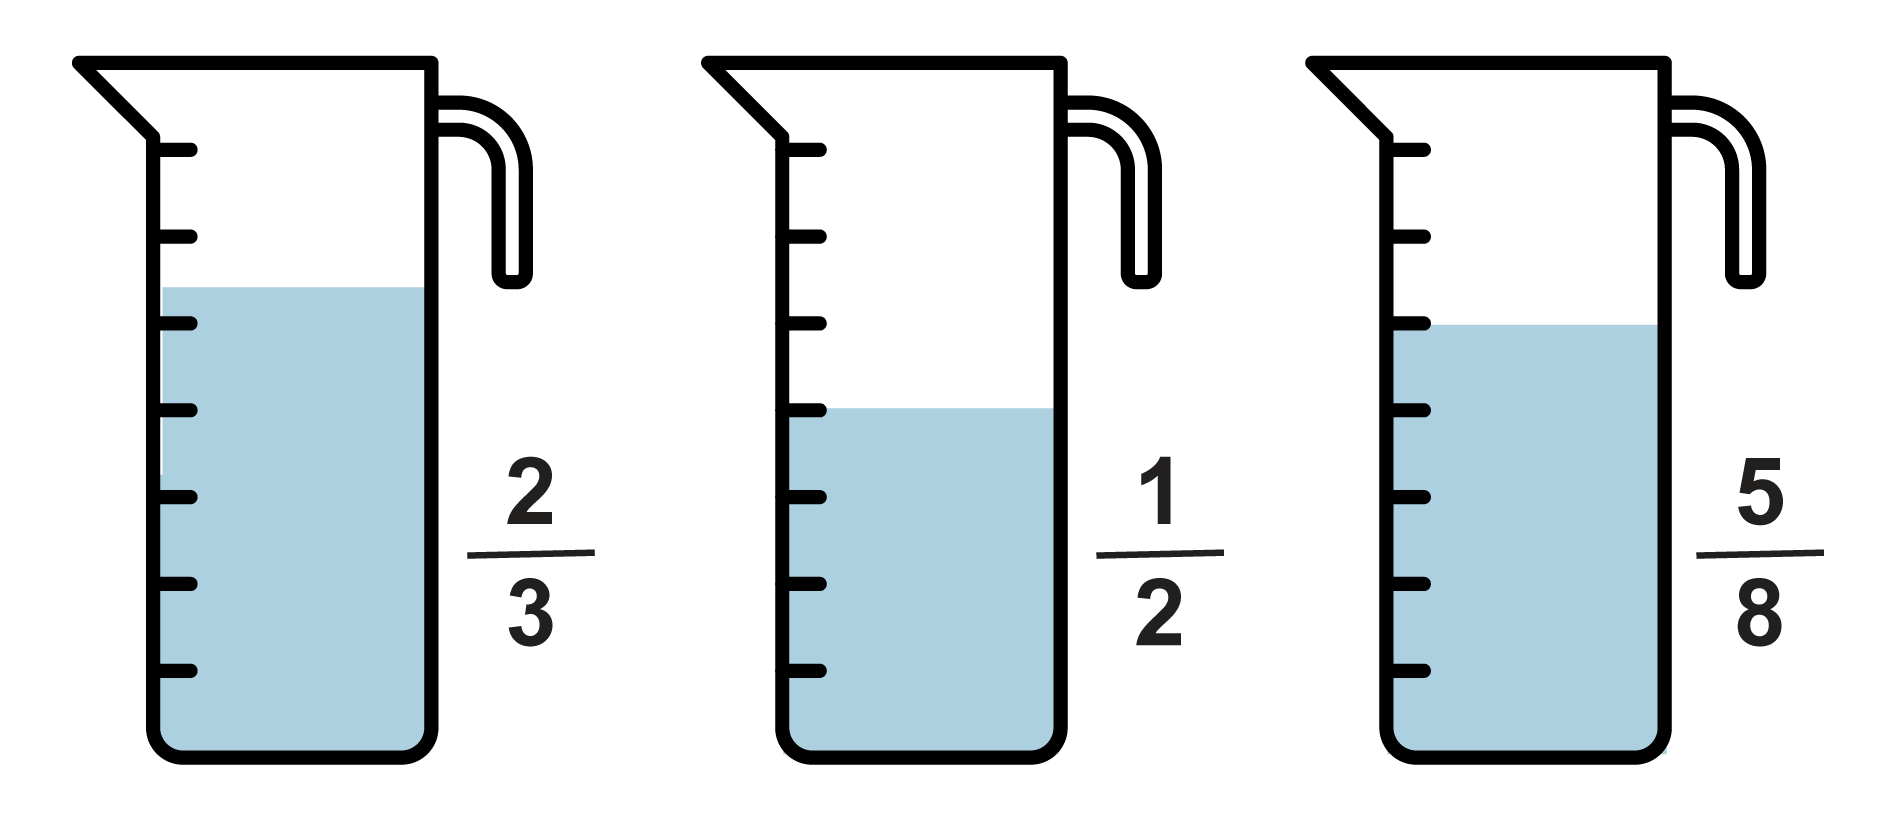
\includegraphics[width=280pt, keepaspectratio]{ativ14_fig01.png}
\end{center}

É possível redistribuir a água de todos os recipientes em somente dois deles?

\ifdefined\prof
\begin{solucao}
  Somando a quantidade de água presente nas três garrafas temos:   $\frac{2}{3}+\frac{1}{2}+\frac{5}{8} = \frac{16}{24}+\frac{12}{24}+\frac{15}{24} = \frac{43}{24}$. Concluímos que é possível, pois   $\frac{43}{24}<\frac{48}{24}=2$.

\end{solucao}
\fi

\end{document}